\chapter{Android}
Facciamo una panoramica su cosa è realmente Android.
Android non è un linguaggio di programmazione, ma un vero e proprio insieme di strumenti e librerie per la realizzazioni di applicazioni mobili.Un aspetto fondamentale del successo di Android è stato il fatto che il linguaggio da esso utilizzato si tratta del ben noto Java. Per rendere, però, eseguibile il codice Java su dispositivi mobili e quindi con risorse hardware limitate sono stati adottati accorgimenti, architetturali e software, per sfruttare al massimo le risorse disponibili.
Il principale cambiamento è stato l'adozione di una nuova Virtual Machine (VM) ottimizzata per l'esecuzione di applicazioni in ambienti a memoria ridotta: la Delvik Virtual Machine (DVM) adottata, infatti, è in grado di eseguire codice contenuto all'interno di file con estensione .dex ottenuti a partire dal byte-code Java con una riduzione di spazio del 50\% . Il Garbage Collector ovvero quella modalità automatica di gestione della memoria che libera le porzioni di memoria non utilizzate è rimasto invariato per non dover lasciare questo compito agli sviluppatori e alleggerirne il lavoro.

\section{L'architettura di Android}
Android ha un'architettura a layer, dove i livelli inferiori offrono servizi ai livelli superiori, che comprende l'insieme degli strumenti per la creazione delle applicazioni per dispositivi mobili, tra cui un sistema operativo, librerie native e Java e una VM dedicata (Figura \ref{fig:architettura-android}).

\begin{figure}[!ht]
  \centering
    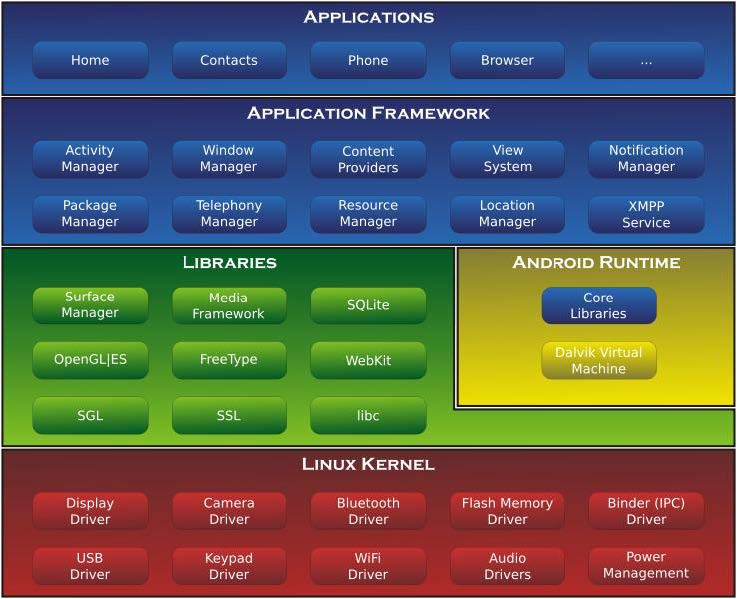
\includegraphics[width=1\textwidth]{architettura-android}
  \caption{Layers architettura Android}
  \label{fig:architettura-android}
\end{figure}
\FloatBarrier
Vediamo ora le sue componenti.

\subsection{Il kernel Linux}
Il livello più basso (in rosso) è occupato dal kernel\footnote{Il kernel costituisce il nucleo di un sistema operativo. Si tratta di un software avente il compito di fornire ai processi in esecuzione sull'elaboratore un accesso sicuro e controllato all'hardware. Dato che possono esserne eseguiti simultaneamente più di uno, il kernel ha anche la responsabilità di assegnare una porzione di scheduling e di accesso all'hardware a ciascun programma (multitasking).} Linux la cui presenza si è ritenuta necessaria per disporre di un vero e proprio sistema operativo che fornisse gli strumenti di basso livello per la virtualizzazione dell'hardware sottostante attraverso driver per la gestione di periferiche di ogni tipo.

\subsection{Librerie native}
Il livello seguente (in verde) è composto da un insieme di librerie standard redatte in C/C++ che rappresentano il core vero e proprio di Android.
\begin{itemize}
\item \textbf{Surface Manager (SM):}  ha il compito di gestire le View (come vedremo in seguito nel capitolo relativo al server) controllando e gestendo le diverse finestre visibili su schermo evitandone, per esempio, la sovrapposizione.
\item \textbf{OpenGL ES:} avendo risorse limitate c'è bisogno di applicare dei cambiamenti anche sul lato della grafica (2D e 3D) e per questo motivo è stato inserito un sottoinsieme delle API dell'OpenGL per semplificare e ottimizzare l'esecuzione delle operazioni di calcolo e rendering.
\item \textbf{SGL:} motore grafico per livelli 2D.
\item \textbf{Media Framework:} contiene le librerie per riprodurre i principali formati audio e video.
\item \textbf{WebKit:} browser-engine che viene integrato in diversi tipi di applicazioni.
\item \textbf{SSL:} librerie per gestire tutti i problemi legati alla sicurezza.
\item \textbf{SQLite:} un potente, ma leggero engine per database relazionali disponibile per tutte le applicazioni.
\item \textbf{FreeType:} librerie per bitmap e vettoriali per font.
\item \textbf{libc:} come si può intuire dal nome, è un'implementazione di librerie C standard, modificate per dispositivi basati su Linux.
\end{itemize}

\subsection{Android Runtime}
È il punto di distinzione tra un sistema operativo Android e un implementazione Linux per dispositivi mobili. È compoto dalla DVM e dalle librerie core che includono gran parte delle funzioni delle librerie standard di Java e ulteriori librerie specifiche per Android. Si occupa della gestione della memoria, della connettività e dei driver necessari al funzionamento di tutto l'ecosistema.

\subsection{Application Framework}
Fornisce i servizi di alto livello alle applicazioni sottoforma di classi Java. Gli sviluppatori sono liberi di utilizzare questi servizi nelle proprie applicazioni.
\begin{itemize}
\item \textbf{Activity Manager:} gestisce il ciclo vitale delle activity nelle applicazioni. Un activity è alla base di qualunque applicazione Android e sostanzialmente consiste nella finestra in cui verrà visualizzata l'interfaccia grafica.
\item \textbf{Content Providers:} gestisce lo scambio di dati tra un'applicazione e l'altra.
\item \textbf{Telephony Manager:} si occupa di tutte le chiamate vocali. Se un applicazione ha necessità di accedere alle chiamate dovrà utilizzare questa componente.
\item \textbf{Location Manager:} fornisce la geolocalizzazione grazie a GPS e ripetitori.
\item \textbf{Resource Manager:} tutti i tipi di risorse di cui un applicazione ha bisogno sono controllate da questo programma.
\item \textbf{Windows Manager:} gestisce le finestre delle diverse applicazioni attive sul dispositivo e relativa visualizzazione.
\item \textbf{Package Manager (PM):} permette alle applicazione di accedere a dati condivisi.
\item \textbf{View System:} fornisce gli strumenti per gestire gli elementi grafici ed arricchirli. Una TextView è per esempio un astrazione della semplice stringa.
\item \textbf{Notification Manager:} permette alle applicazioni di interagire con l'utente tramite notifiche.
\end{itemize}

\subsection{Applications}
L'ultimo livello è occupato dalle applicazioni installate nel sistema, siano esse native o di terze parti. Android non fa differenza tra applicazioni native e quelle provenienti da altre fonti garantendo ad entrambe gli stessi privilegi.

\section{Activity}

\begin{wrapfigure}{r}{0.4\textwidth}
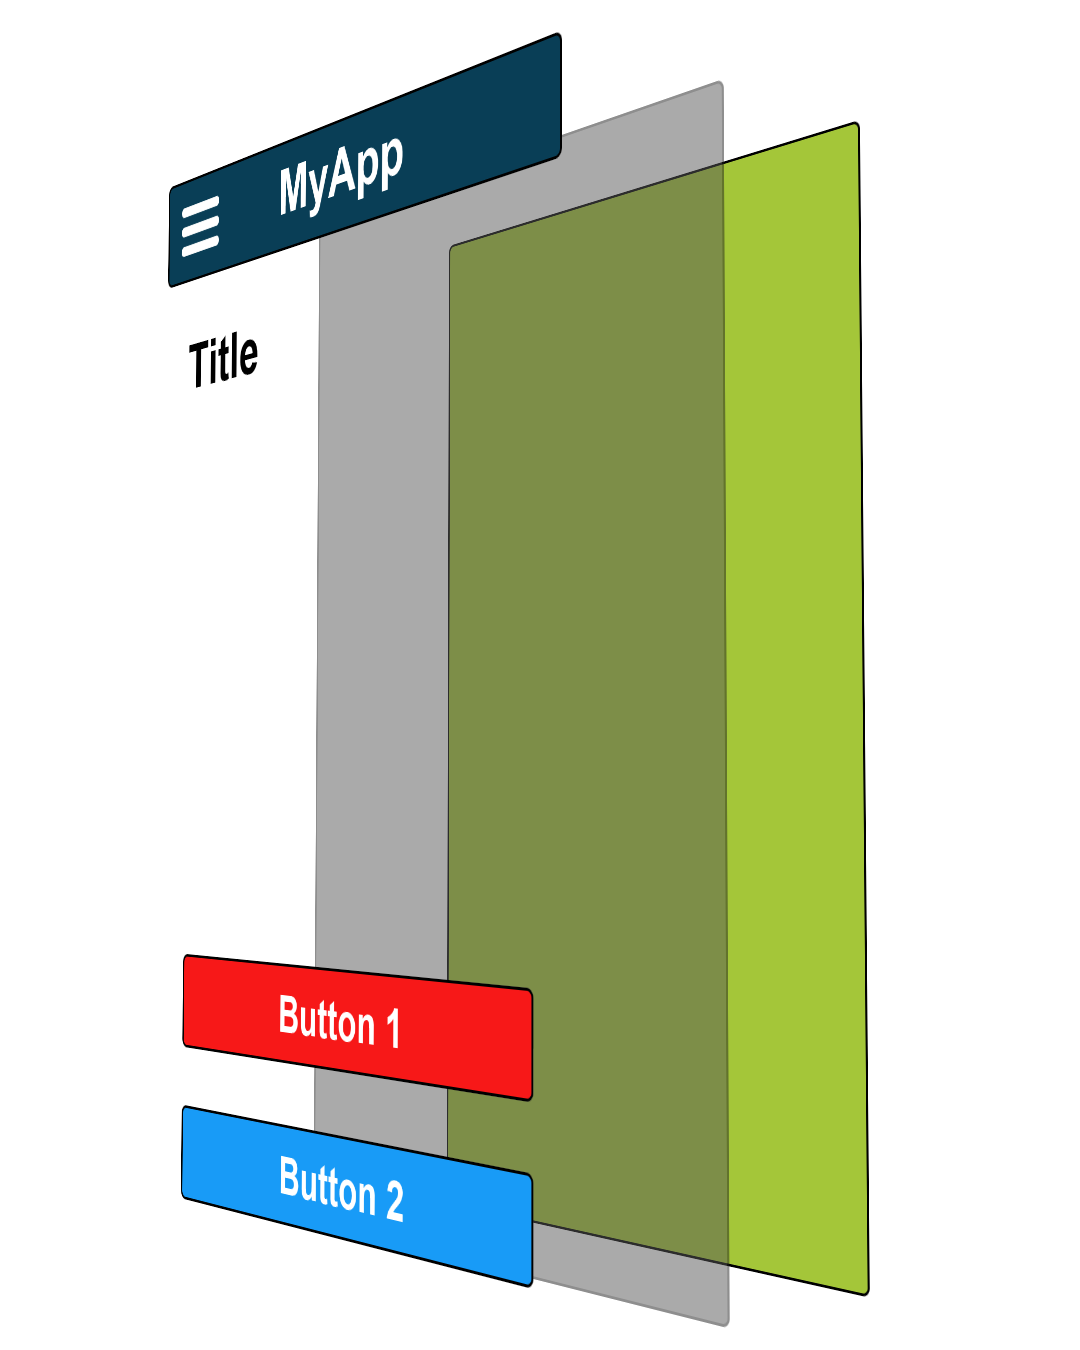
\includegraphics[width=0.4\textwidth]{activity}
\caption{View in Android}
\label{fig:activity}
\end{wrapfigure} 
\FloatBarrier

Parleremo nel capitolo seguente del paradigma MVC durante la descrizione del server, ma anticipiamo ora la sua descrizione lato client.
Sul client ci occuperemo solo della View (che scopriremo poi essere la parte interattiva di un sistema MVC).
Possiamo vedere il client come una sorta di telecomando che impartisce ordini al computer remoto che è il server.
La View di Android è chiamata Activity ed è alla base di ogni applicazione.
L'activity si occupa di creare la finestra nella quale lo sviluppatore inserirà il codice per l'interfaccia utente e di interpretare le azioni dell'utente in comandi da eseguire.
Da Android 3.0 si è aggiunta un'altra entità a sostegno dell'activity: il Fragment. I fragments sono una sorta di classe figlia della classe Activity e ne condividono gran parte del ciclo vitale (non può esistere un Fragment senza la sua activity). Essendo più "leggeri" di un activity a livello computazionale, più fragments possono coesistere sulla stessa activity contemporaneamente o sostituirsi tra loro.
In sostanza un'applicazione è composta come in Figura \ref{fig:activity}: in verde è rappresentata l'activity principale (un'applicazione può comunque passare da un'activity ad un altra a seconda dei casi) che gestirà le funzioni basilari dell'applicazione; sopra l'activity troviamo il fragment (in grigio): ogni fragment è una componente a sè stante che possiede le sue funzioni e relativo layout.
L'ultimo strato è appunto occupato dal Layout, ovvero la parte visibile ad occhio nudo, scritto in linguaggio XML associato a classi CSS.